\newcommand{\NWtarget}[2]{#2}
\newcommand{\NWlink}[2]{#2}
\newcommand{\NWtxtMacroDefBy}{Fragment defined by}
\newcommand{\NWtxtMacroRefIn}{Fragment referenced in}
\newcommand{\NWtxtMacroNoRef}{Fragment never referenced}
\newcommand{\NWtxtDefBy}{Defined by}
\newcommand{\NWtxtRefIn}{Referenced in}
\newcommand{\NWtxtNoRef}{Not referenced}
\newcommand{\NWtxtFileDefBy}{File defined by}
\newcommand{\NWtxtIdentDefinedIn}{defined in}
\newcommand{\NWtxtIdentUsedIn}{used in}
\newcommand{\NWtxtIdentUsers}{Users:}
\newcommand{\NWtxtIdentsNotUsed}{never used}
\newcommand{\NWtxtIdentsUsed}{Uses:}
\newcommand{\NWsep}{${\diamond}$}
\newcommand{\NWnotglobal}{(not defined globally)}
\newcommand{\NWuseHyperlinks}{}
\documentclass[a4paper, 12pt]{article}
\usepackage{fullpage} % for 1.5 cm margins
\renewcommand{\familydefault}{\sfdefault} % so it doesn't look like LaTeX
\usepackage{helvet}
\usepackage{graphicx}
\graphicspath{ {imgs/} }
\usepackage{float} % so the figures stay with the text


\usepackage{abstract}
\renewcommand{\abstractname}{Overview}
\raggedright

\usepackage{parskip}

\usepackage{hyperref}
\hypersetup{
    colorlinks=true,
    linkcolor=blue,
    filecolor=magenta,      
    urlcolor=cyan,
}

\title{Promethean Temperature Sensor}
\author{Joe J Collins}

\begin{document}
\maketitle
%%%%%%%%%%%%%%%%%%%%%%%%%%%%%%%%%%%%%%%%%%%%%%%%%%%%%%%%%%%%
\tableofcontents


%%%%%%%%%%%%%%%%%%%%%%%%%%%%%%%%%%%%%%%%%%%%%%%%%%%%%%%%%%%%
\section{The Problem}

Monitoring with Prometheus
no off the shelf monitoring.
Temperature is important.

No hassle with Wifi.

\begin{description}
  \item[Start up time]
  \item[Maintenance]
  \item[Cost]
  \item[Availability]
  \item[Support information] 
\end{description}


%%%%%%%%%%%%%%%%%%%%%%%%%%%%%%%%%%%%%%%%%%%%%%%%%%%%%%%%%%%%
\section{Components}

Shopping list and details, with prices.

\begin{figure}[H]
  \centering
  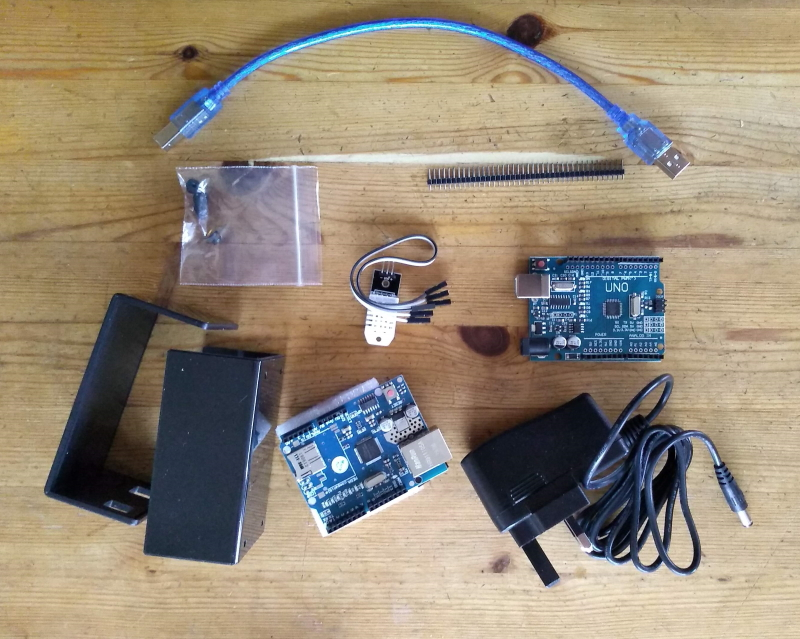
\includegraphics[width=0.8\textwidth]{components.jpg}
  \caption{Components}
\end{figure}


\begin{tabular}{ll}
  \textbf{Component} & \textbf{Cost} \\ 
  \hline
  Arduino Uno Rev3, ATmega328P, CH340G Compatible Board & \pounds 5.79 \\
  UK 9V AC/DC Power Supply Adapter Plug for Arduino Uno & \pounds 7.95 \\
  Ethernet Shield LAN W5100 for Arduino Uno & \pounds 7.75 \\
  DHT22 AM2302 Digital Temperature and Humidity Sensor & \pounds 6.90 \\
  1/4W 0.25W Metal Film Resistor 10K Ohm & \pounds 0.99 \\
  Uno Ethernet Shield Case & \pounds 10.36 \\
  \hline
  Total cost in November 2020 & \textbf{\pounds 39.74}  \\
\end{tabular}

\subsection{Sensor}

AM2302 capacitive humidity sensing digital temperature and humidity module is one that contains the
compound has been calibrated digital signal output of the temperature and humidity sensors. 

\begin{flushleft} \small
\begin{minipage}{\linewidth}\label{scrap1}\raggedright\small
\NWtarget{nuweb2}{}$\langle\,${\itshape configuration}\nobreak\ {\footnotesize{2}}$\,\rangle\equiv$
\vspace{-1ex}
\begin{list}{}{\setlength{\leftmargin}{1em}} \item
\mbox{}\verb@  #define DHTPIN 2@\\
\mbox{}\verb@  // Set DHT type, uncomment whatever type you're using!@\\
\mbox{}\verb@  //#define DHTTYPE DHT11   // DHT 11 @\\
\mbox{}\verb@  #define DHTTYPE DHT22   // DHT 22  (AM2302)@\\
\mbox{}\verb@  //#define DHTTYPE DHT21   // DHT 21 (AM2301)@\\
\mbox{}\verb@  // Initialize DHT sensor for normal 16mhz Arduino:@\\
\mbox{}\verb@  DHT dht = DHT(DHTPIN, DHTTYPE);@\\
\mbox{}{\NWsep}
\end{list}
\vspace{-1ex}
\vspace{-1ex}
\footnotesize
\begin{list}{}{\setlength{\itemsep}{-\parsep}\setlength{\itemindent}{-\leftmargin}}
\item \NWtxtMacroRefIn\ \NWlink{nuweb4a}{4a}.
\end{list}
\end{minipage}
\end{flushleft}


%%%%%%%%%%%%%%%%%%%%%%%%%%%%%%%%%%%%%%%%%%%%%%%%%%%%%%%%%%%%
\section{Wiring}

Pull up resistor.



\begin{figure}[H]
  \centering
  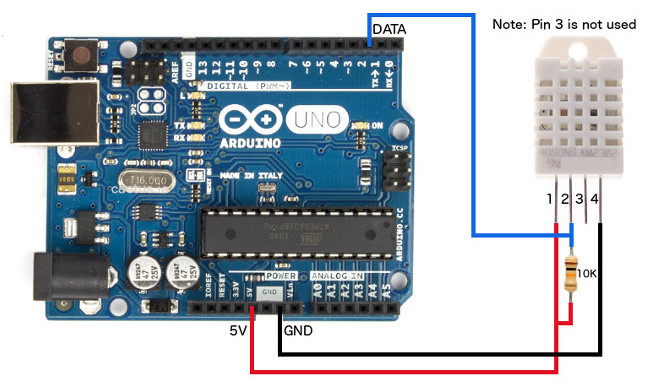
\includegraphics[width=0.8\textwidth]{wiring-dht22.jpg}
  \caption{Wiring diagram with pull up resistor}
\end{figure}



%%%%%%%%%%%%%%%%%%%%%%%%%%%%%%%%%%%%%%%%%%%%%%%%%%%%%%%%%%%%
\section{Programming}

Rather than link up to a router

\begin{itemize}
  \item Assign a manual IP address to the laptop's ethernet connection say 10.0.21.1.
  \item Subnet mask 255.255.255.0.
  \item Assign a manual IP address to the Arduino's ethernet, say 10.0.21.211.
  \item Subnet mask 255.255.255.0.
  \item Leave the default Gateway empty.
  \item Use an ethernet patch cable to link the two (since 100BaseT onwards it doesn't have to be a special cross over cable).
  \item You should then be able to get your Arduino site up on http://192.168.0.2 from the laptop.
\end{itemize}


Platform io

\begin{flushleft} \small
\begin{minipage}{\linewidth}\label{scrap2}\raggedright\small
\NWtarget{nuweb4a}{}\verb@"../src/shit.cpp"@\nobreak\ {\footnotesize{4a}}$\equiv$
\vspace{-1ex}
\begin{list}{}{\setlength{\leftmargin}{1em}} \item
\mbox{}\verb@#include <Arduino.h>@\\
\mbox{}\verb@@$\langle\,${\itshape libraries}\ {\footnotesize \NWlink{nuweb4b}{4b}}\,$\rangle\,$\verb@@\\
\mbox{}\verb@@$\langle\,${\itshape configuration}\ {\footnotesize \NWlink{nuweb2}{2}}\,$\rangle\,$\verb@@\\
\mbox{}\verb@void setup() @\\
\mbox{}\verb@{@\\
\mbox{}\verb@  @$\langle\,${\itshape setup}\ {\footnotesize (not found)}\,$\rangle\,$\verb@@\\
\mbox{}\verb@}@\\
\mbox{}\verb@void loop() @\\
\mbox{}\verb@{@\\
\mbox{}\verb@  @$\langle\,${\itshape loop}\ {\footnotesize (not found)}\,$\rangle\,$\verb@@\\
\mbox{}\verb@}@\\
\mbox{}{\NWsep}
\end{list}
\vspace{-1ex}
\end{minipage}
\end{flushleft}


%%%%%%%%%%%%%%%%%%%%%%%%%%%%%%%%%%%%%%%%%%%%%%%%%%%%%%%%%%%%
\subsection{Libraries}

Notes

\begin{flushleft} \small
\begin{minipage}{\linewidth}\label{scrap3}\raggedright\small
\NWtarget{nuweb4b}{}$\langle\,${\itshape libraries}\nobreak\ {\footnotesize{4b}}$\,\rangle\equiv$
\vspace{-1ex}
\begin{list}{}{\setlength{\leftmargin}{1em}} \item
\mbox{}\verb@// Include the libraries:@\\
\mbox{}\verb@#include <Adafruit_Sensor.h>@\\
\mbox{}\verb@#include <DHT.h>@\\
\mbox{}\verb@#include <SPI.h>@\\
\mbox{}\verb@#include <Ethernet.h>@\\
\mbox{}{\NWsep}
\end{list}
\vspace{-1ex}
\vspace{-1ex}
\footnotesize
\begin{list}{}{\setlength{\itemsep}{-\parsep}\setlength{\itemindent}{-\leftmargin}}
\item \NWtxtMacroRefIn\ \NWlink{nuweb4a}{4a}.
\end{list}
\end{minipage}
\end{flushleft}


%%%%%%%%%%%%%%%%%%%%%%%%%%%%%%%%%%%%%%%%%%%%%%%%%%%%%%%%%%%%
\subsection{Upload}

Drivers on PC.



%%%%%%%%%%%%%%%%%%%%%%%%%%%%%%%%%%%%%%%%%%%%%%%%%%%%%%%%%%%%
\subsection{Testing}

\begin{verbatim}
  --- Quit: Ctrl+C | Menu: Ctrl+T | Help: Ctrl+T followed by Ctrl+H ---
  Webserver set up
  Sensor set up
  Humidity: 55.90 % | Temperature: 22.10 C
  Humidity: 56.30 % | Temperature: 22.20 C
  \end{verbatim}
  
  This is the endpoint at \url{http://10.0.21.211/}.
  
  \begin{verbatim}
    > curl 10.0.21.211
    # HELP temperature is the last temperature reading in degrees celsius
    # TYPE temp gauge
    temperature 23.30
    # HELP humidity is the last relative humidity reading as a percentage
    # TYPE humidity gauge
    humidity 47.60
  \end{verbatim}

%%%%%%%%%%%%%%%%%%%%%%%%%%%%%%%%%%%%%%%%%%%%%%%%%%%%%%%%%%%%
\section{Packaging}

\begin{figure}[H]
  \centering
  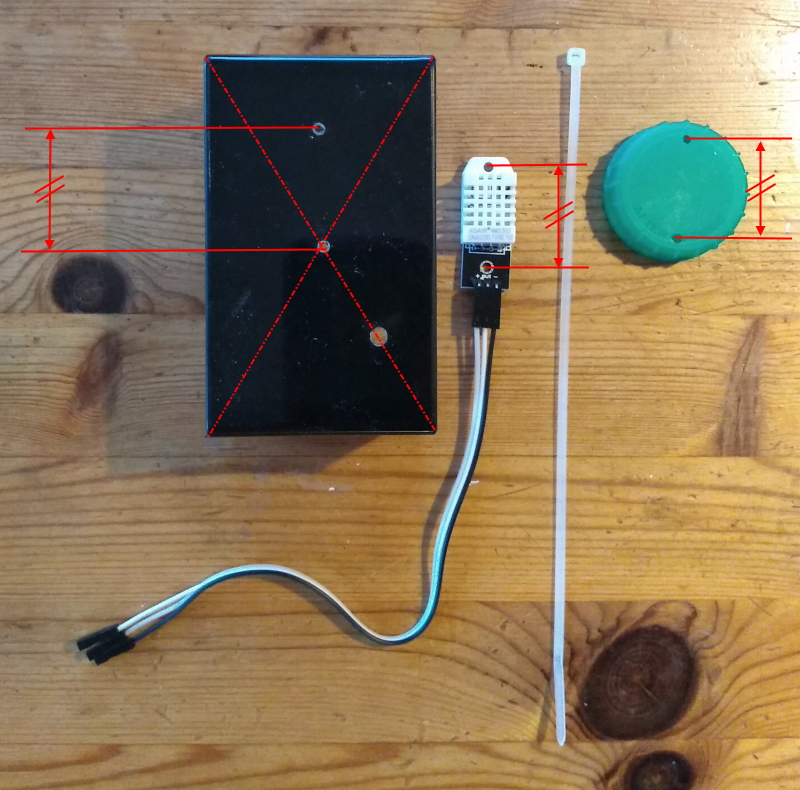
\includegraphics[width=0.8\textwidth]{sensor-mount.jpg}
  \caption{Components for mounting the sensor}
\end{figure}



2.5 mm holes and 4 mm holes.

\begin{figure}[H]
  \centering
  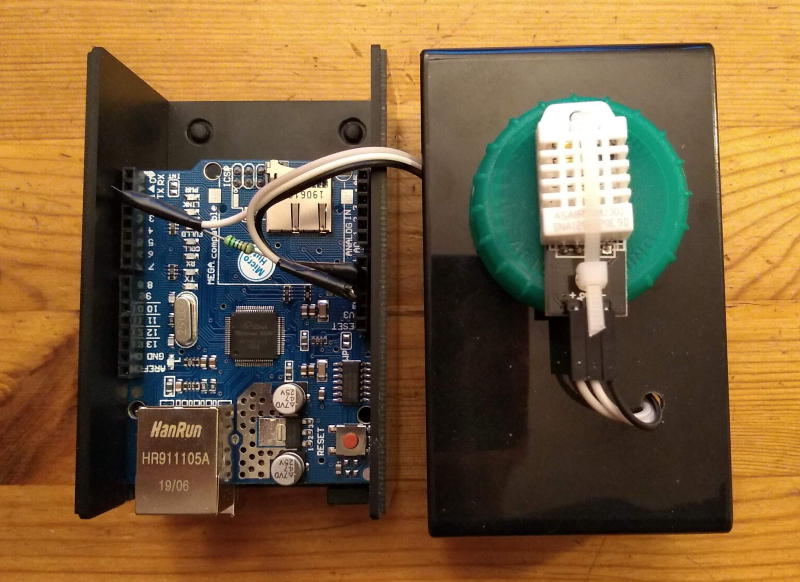
\includegraphics[width=0.8\textwidth]{packaging.jpg}
  \caption{Mounted sensor and wiring}
\end{figure}

\end{document}